\chapter{Bienestar Animal e Historia Clínica Veterinaria}\label{chapter:animalHealth}

\section{Bienestar Animal}
El bienestar animal es un concepto amplio que incluye diversos elementos que contribuyen a la calidad de vida de un animal, incluidos los referidos en las “cinco necesidades” (libertades) \brackcite{manteca2012bienestar}: 
\begin{itemize}
\item necesidad de no sufrir hambre, sed ni desnutrición,
\item necesidad de no experimentar miedo ni angustia
\item necesidad de vivir libre de incomodidad física y térmica,
\item necesidad de no sufrir de dolor, lesiones y enfermedad,
\item y necesidad de expresar patrones normales de comportamiento.
\end{itemize}

Ha sido definido por la Organización Mundial de Sanidad Animal (OIE) como el término que describe la manera en que los animales se enfrentan con el medio ambiente y que incluye su sanidad, sus percepciones, su estado anímico y otros efectos positivos o negativos que influyen sobre los mecanismos físicos y psíquicos del animal \brackcite{manteca2012bienestar}.

Por otra parte, el biólogo y profesor de bienestar animal Donald Broom lo describe como: “\textit{el equilibrio del estado físico y psicológico de un animal en su intento por adaptarse y sobrevivir en las condiciones de su entorno o medio ambiente}” \brackcite{broom2017animal}. Para Dawkins \brackcite{dawkins2016animal} el animal vive con un adecuado bienestar cuando “\textit{está sano y tiene lo que quiere}”. Teniendo en cuenta la bibliografía consultada se puede concluir que el bienestar animal se refiere al estado de felicidad que experimenta un individuo al adaptarse de manera exitosa y positiva ante los cambios del entorno, logrando suplir sus necesidades, lo cual involucra la salud y el confort.

 A continuación, se muestra una lista planteada por Blasco \brackcite{blasco2011etica} que describe de manera general las principales formas de relación humano-animal a través de la historia:
\begin{enumerate}
\item Cría de animales en granja para consumir sus productos (leche, huevo, etc.).
\item  Cría y matanza de animales para consumir su carne.
\item  Cautiverio de animales fuera de sus ambientes naturales con fines de esparcimiento (zoológicos, circos, parques, etc.).
\item  Deporte (caza, pesca).
\item  Experimentación con animales.
\item  Animales de compañía.
\item  Animales usados para trabajo (guarda, transporte).
\item  Espectáculos con animales amaestrados (acuarios, circos, etc.).
\item  Espectáculos que involucran agresividad hacia los animales (tauromaquia, pelea de gallos, pelea de perros, etc.).
\item  Tratamiento de plagas (ratas, conejos, insectos, etc.).
\end{enumerate}
En la actualidad, desafortunadamente, la gran demanda de productos ha ocasionado el aumento de sistemas intensivos de producción animal que atentan contra el bienestar de los mismos. Ciertas especies animales son explotadas y consideradas como meras máquinas de producción, sin tener en cuenta que son seres que sufren de manera física y emocional. Es por ello que hoy en día se han desarrollado una serie de políticas y prácticas para protegerlos. 

Según Giménez \brackcite{gimenez2014animales} la sociedad demanda, cada día más, no solo que los animales domésticos reciban un trato digno y que no proliferen los abandonos y maltratos, sino que se beneficien de una consideración cada vez mayor, que reciban un trato adecuado a su condición de seres vivos sensibles y que la concepción misma del animal como objeto del Derecho alcance una mayor coherencia jurídica. Este sentir colectivo se ha venido mostrando, fundamentalmente, en el desarrollo de legislaciones y marcos normativos para funcionar como vía de la protección estatal de los animales y sus posibles derechos, tanto en Europa y Estados Unidos, como en América Latina.  

En el caso de Cuba, fue aprobado en febrero del año 2021 el Decreto-Ley No.31 de Bienestar Animal, lo cual constituye un paso de avance en el empeño de proteger a los animales. Esta ley regula los principios, deberes, reglas y fines respecto al cuidado, la salud y la utilización de estos individuos para garantizar su bienestar. El Ministerio de Salud Pública del país (MINSAP) dispone de programas de vigilancia, prevención y control de enfermedades zoonóticas, enfocados en aquellas que constituyen un riesgo para la salud. Para cumplir con los objetivos de estos programas se realizan diversas acciones como el monitoreo de la ocurrencia de casos, diagnóstico microbiológico, control de focos, atención médica a las personas, vacunación de grupos de riesgo y poblaciones de animales, educación sanitaria y promoción de salud. \brackcite{Minsap2022Feb}

\textbf{En el Anexo 1 del presente trabajo se muestra una tabla con la relación del marco normativo existente en otros países de América que hacen referencia a la protección de los animales.} 

La promulgación sistemática de leyes que protegen a estos seres vivos y prohíben prácticas violentas e innecesarias en contra de su vida y dignidad, evidencia una tendencia al reconocimiento y la protección normativa del derecho al bienestar de los animales \brackcite{jarrin2021diseno}. Sin lugar a dudas, la sociedad se halla cada vez más preocupada por el cuidado de los mismos; lo cual ha conllevado a la generación de nuevas tecnologías para optimar los servicios de atención a los animales. Es en este punto donde se inscribe el presente trabajo mediante el cual se intenta desarrollar una herramienta para conservar de forma segura y conveniente el historial médico de animales afectivos. Esta herramienta, en forma de aplicación móvil con respaldo de datos en un servidor, será de ayuda tanto a propietarios de mascotas como a médicos veterinarios en la consecución de un mayor bienestar de los animales bajo su cuidado. 

\section{Antecedentes históricos de los servicios veterinarios}

Según la OIE los servicios veterinarios se refieren a las organizaciones, gubernamentales o no, que aplican las medidas de protección de la sanidad, el bienestar de los animales y las demás normas y recomendaciones del Código Terrestre y del Código Sanitario para los Animales Acuáticos de la OIE en el territorio de un país. Los Servicios Veterinarios actúan bajo control y tutela de la autoridad veterinaria. Normalmente, las organizaciones del sector privado, los profesionales veterinarios o los profesionales de la sanidad de los animales acuáticos deben contar con la acreditación o aprobación de la autoridad veterinaria para ejercer estas funciones delegadas \brackcite{depapel}. 

Acorde a lo planteado por \brackcite{Fernandez2004} la práctica de la cirugía veterinaria se remonta a épocas ancestrales. Desde la edad primitiva el hombre atendía a los animales con los cuales convivía. Evidencias de ello existen en las pinturas halladas en la gruta de Altamira, en Santander, España, donde se admiran diseños de instrumentos de cirugía que datan de más de 2500 años a.n.e. y que fueron utilizados para realizar una operación cesárea a un bisonte hembra.   

Los primeros antecedentes sobre la preocupación por el cuidado y la sanación de los animales se remontan al mundo mesopotámico. En Babilonia, aproximadamente en el 1.700 años a.C., en el famoso Código del Rey Hammurabi (primer conjunto de leyes de la historia) aparecen referencias a la actividad pecuaria y a la acción del curador de los animales. Así también, los caldeos poseían un amplio conocimiento sobre producción animal y tratamientos médicos para los animales. En el año 1.500 a.n.e se registra el hallazgo de un tratado de cura de animales en Ugarit, ciudad ubicada en la costa mediterránea al norte de Siria, en el que se expone el tratamiento de los equinos enfermos y débiles \brackcite{dunlop1996veterinary}. 

De este modo, numerosos son los hechos que demuestran la presencia de los servicios veterinarios a través de la historia. En la cultura egipcia, durante el período del Reino Nuevo (1.500 – 1.000 años a.C.), los sacerdotes cuidaban de los animales y les hacían curaciones o daban medicamentos naturales para tratar enfermedades . Por su parte, fueron los árabes, durante la Edad Media, quienes desarrollaron las prácticas de diagnóstico y tratamiento de enfermedades del hombre y los animales. No obstante, estos se preocupaban principalmente de solucionar problemas prácticos antes que entender el concepto del proceso íntimo de la enfermedad \brackcite{perez2008recopilaciones}.  

Durante el período de influencia del pensamiento ilustrado, en 1761, se fundó y se puso en funcionamiento la Escuela de Veterinaria de Lyon, la primera institución educativa en esta especialidad en el mundo. El destacado Veterinario francés Claude Bourgelat (1712 – 1779) en el mismo año publica Eléments de l’art vétérinaire, obra fundadora de una verdadera Veterinaria científica, y es nombrado director de la recién creada Escuela Nacional Veterinaria de Lyon. Bourgelat es considerado como el fundador de la medicina equina en Francia y en 1776 participa en la fundación de Escuela Nacional de Veterinaria de Maisons-Alfort en París. \brackcite{thesisSistemaInf} 

Hasta principios de la segunda mitad del siglo XIX, los veterinarios del continente americano eran graduados de escuelas españolas, francesas o de otros países europeo. La carencia de escuelas especializadas en los países del continente produjo que durante un largo período fueran enviados veterinarios, principalmente de Europa hacia América.  

Algunos de los acontecimientos más importantes de esta etapa fueron \brackcite{desarrolloMedVet}: 
\begin{itemize}
 \item El establecimiento de la “Primera Escuela de Veterinaria Moderna”, por Claude Burgelat en Lyon, Francia, el 1ro de enero de 1762 y 2 años después en 1764, la de Alfort.  
 \item En España se fundó la “1ra Escuela de Medicina Veterinaria” el 23 de febrero de 1792.  
 \item  La “Primera Escuela de Veterinaria” en América se fundó en 1853 en San Jacinto, México. En 1885 Viricel fundó la Escuela de Veterinaria de Colombia, Bogotá  
\end{itemize}
\newpage

\subsection{Historia de la Veterinaria en Cuba}

En Cuba al finalizar la etapa colonial existía un gran atraso en la veterinaria, cuando existían ya en el mundo 37 escuelas dedicadas a ello. No fue hasta el año 1868 que se logró fundar la “Real Academia de Ciencias Médicas, Físicas y Naturales de la Habana”, institución compuesta por académicos numerarios, corresponsales y de mérito.  

En abril de 1907 se estableció la “Escuela Libre de Medicina Veterinaria”, que quedó ubicada en la esquina de Zanja y Belascoain, Centro Habana, en la capital de la República. La misma fue adscrita, meses después, a la Facultad de Medicina y Farmacia de la Universidad de la Habana mediante Decreto No. 126 del 21 de enero de 1908. Tras ser inaugurada, comenzaron a laborar los primeros veterinarios cirujanos que constituyeron la “Primera Generación”, los cuales debieron encargarse de la resolución de los problemas quirúrgicos del pie del caballo, animal muy preciado en aquel entonces \brackcite{desarrolloMedVet}.  

Luego del triunfo revolucionario, se produjeron cambios radicales en el Sistema de la Medicina Veterinaria en Cuba que han permitido su avance. Tanto los ocurridos en la docencia, la producción, como en los servicios y la investigación, permitieron erradicar la peste porcina africana, en los años 1971 y 1980. Asimismo, el control de la brucelosis en un 98\% de la masa bovina, el 90\% de la bufanina, y en la totalidad del ganado ovino-caprino de todos los sectores productivos. \brackcite{grammaArticle} A partir de 1959, se constituyen las cátedras de cirugía  de la etapa revolucionaria en los diferentes centros universitarios agropecuarios del país. Los profesores que pertenecieron a las mismas contribuyeron a la confección de los libros de textos y guías de cirugía, realizaron nuevos aportes y modificaciones a las técnicas quirúrgicas, algunos de ellos han brindado también su aporte solidario en países de Asia, África y América Latina. 

\section{La historia clínica}

La historia clínica (HC) es el documento que avala legalmente el trabajo del médico, pues en ella se expresan los resultados obtenidos en el diagnóstico clínico, y sirve de apoyo para el planeamiento, ejecución y control en cada caso, de las acciones destinadas a la recuperación y rehabilitación de la salud del paciente. Aunque en el presente trabajo se trata la HC veterinaria muchos de los planteamientos en esta sección se derivan de la HC para humanos ya que ambas poseen muchas características similares. 

Para \brackcite{gonzalez2015historia} la HC es un instrumento mediador a través del cual el médico elabora el diagnóstico, fundamenta el pronóstico, consigna el tratamiento y la evolución del paciente, siendo un documento único, integrado y acumulativo para cada persona. La existencia de normas y leyes que hacen obligatorio su empleo, argumentan desde el punto de vista jurídico y normativo sus usos en lo asistencial, formativo y docente, científico e investigativo, evaluador de la calidad asistencial, administrativo y jurídico legal. De esta forma, la HC se convierte en el soporte escrito sobre el cual quedan las evidencias de la atención médica integrada que hacen todos los profesionales y técnicos de la salud partícipes en la misma \brackcite{odio2019historia}. 

El profesor cubano Llanio Navarro la considera como una guía metodológica para la identificación integral de los problemas de salud de cada persona que establece todas sus necesidades. Es fundamental para analizar el proceso patológico del paciente y su evolución. A partir de lo expresado, toda la información que se obtiene con exactitud en la inspección médica debe ser registrada en un documento llamado HC \brackcite{cuenca2014historia}. La información contenida en la HC puede obtenerse por diferentes vías: la anamnesis, información surgida de la entrevista clínica proporcionada por el dueño del paciente; la exploración física o clínica; pruebas o exámenes complementarios realizados por el médico; juicios de valor que el propio médico extrae de documentos que él elabora para fundamentar un diagnóstico, prescribir el tratamiento y finalmente dejar constancia del curso de la enfermedad y el método instaurado. Los componentes principales de la HC son: datos subjetivos proporcionados por el dueño del paciente; datos objetivos obtenidos de la exploración física y de las exploraciones complementarias; diagnóstico; pronóstico y tratamiento. \brackcite{garcia2006historia}   

La HC es única para cada paciente, este último es sujeto de su propia investigación, la cual comienza con el diagnóstico de su enfermedad. Cabe agregar que por razones económicas y gerenciales la HC debe estar siempre disponible y facilitarse en los casos legalmente contemplados, resguardando la confidencialidad de los datos reflejados en ella. El acceso al expediente clínico sin autorización, en detrimento de un tercero, está catalogado como delito.

Se advierte que el redactar datos y argumentaciones en la historia clínica es una responsabilidad de los médicos (veterinarios) de atención, sobre la cual podrían, luego de un tiempo, sustentar sus propias evidencias defensivas ante posibles denuncias concernientes a su responsabilidad profesional. En Cuba la historia clínica es propiedad del hospital con un plazo de conservación y custodia de cinco años. Por lo cual, es conveniente recordar que cada actuación profesional que se realice debe ser datada con el tiempo y lugar donde se realiza, firmada, sellada con su cuño profesional y con las aclaraciones precisas sobre el acto ejercido   \brackcite{santana2016proposito}.

De acuerdo a las características expresadas previamente sobre la HC, se puede intuir la gran importancia que adquiere para brindar un tratamiento acertado al paciente. Se tendrá que dedicar tiempo, capacidad de observación, juicio clínico, creatividad, capacidad para analizar situaciones nuevas, prudencia y rigor científico a fin de lograr su correcta confección. En este sentido, una HC ilegible y desordenada, perjudica tanto a médicos como a todo personal sanitario que necesite de su consulta, además de contribuir desfavorablemente al proceso evolutivo del paciente. El proceso asistencial y docente puede dificultarse por los errores que se deriven de una inadecuada interpretación de los datos clínicos.  

La HC puede presentarse en diferentes soportes: Papel que tradicionalmente ha sido manuscrito, teniendo inconvenientes para la legibilidad de la caligrafía por el volumen de espacio que ocupa y el deterioro con el paso del tiempo, videos, fotografías, estudios radiológicos y soporte informático. En los nuevos centros de atención médica y veterinaria las historias clínicas están informatizadas, mediante complejos sistemas informáticos \brackcite{garcia2006historia}.

En los últimos años, el auge de las tecnologías de la información y las comunicaciones (TIC) ha propiciado el incremento de su empleo en los servicios médicos. Así, se ha desarrollado la Historia Clínica Informatizada (HCI), donde el término informatizada se refiere a la técnica que, mediante sistemas electrónicos, y programas informáticos permiten un manejo de la información cumpliendo con las condiciones ideales para el manejo documental y asistencial de los expedientes sanitarios  \brackcite{garay}. La HCI recopila la información referente a lo que se pensó, dijo o se hizo acerca del paciente mediante un dispositivo electrónico  \brackcite{garcia2006historia}.

Los criterios brindados por diferentes investigadores del tema como  \brackcite{elorza2012estudio} , \brackcite{thesisSistemaInf}  y \brackcite{hidalgo} coinciden en que la HCI es el conjunto global y estructurado de información, vinculado a los procesos de la asistencia médico-sanitaria de los pacientes, soportado en una plataforma informática para cumplir con las expectativas de los usuarios. 

La sustitución de la HC tradicional (en soporte papel) por la HCI responde a varias necesidades \brackcite{rueda2006historia}:  

\begin{enumerate}
	\item Dar cumplimiento a las características y objetivos del documento HC en cuanto a los requerimientos del equipo sanitario, manteniendo la confidencialidad.  
	
	\item Resolver los dos problemas clásicos de los archivos de HC el almacenamiento de grandes volúmenes documentales y la seguridad frente a los riesgos de pérdida y de deterioro.  
	
	\item Permitir la transferencia rápida de la información sanitaria existente de un paciente a puntos lejanos, garantizando que cada paciente solo tenga un único expediente y este pueda ser consultado simultáneamente en distintos lugares.  
	
	\item Soportar las decisiones médico-asistenciales, mediante la interacción con bases de datos, que permitan una rápida consulta de las mejores prácticas, los protocolos de manejo y las evidencias reconocidas.  
	
	\item Poner a disposición de los educadores, investigadores y de los planificadores sanitarios esta información, en forma eficiente. 
\end{enumerate}

La calidad en su confección está condicionada por muchos factores. Por un lado, está el nivel de exigencia en las instituciones; por otro, el nivel de aprendizaje de los que la confeccionan. Los problemas que puedan suscitar en su confección, pueden ser atribuidos al desconocimiento, beneficios o perjuicios derivados de un contenido incompleto  \brackcite{garcia2006historia}.

En la figura \ref{HCIvsHC} se resumen las diferentes características de la HC tradicional y la HCI a través de una comparación de sus fortalezas y debilidades.

Los programas para el manejo de la información de la HC principalmente tienen dos componentes: una base de datos y un programa informático para suministrar y acceder a estos datos. Por el volumen de información que se maneja cada uno de estos componentes debe tener la potencia y la seguridad que garanticen un adecuado producto. Hoy son innumerables los programas y soluciones informáticas que se ofrecen en el mercado, lo cual ha generado gran cantidad de soluciones, adecuadas a los requerimientos y las exigencias de sus creadores \brackcite{rueda2006historia}. El propio autor señala que los factores que con mayor peso influyen negativamente en la adopción e implementación a nivel institucional de la HCI son:  

\begin{itemize}
\item	Los desarrollos estandarizados (comerciales) no siempre cumplen las expectativas de los usuarios lo que genera mayor resistencia al cambio.  
	
	\item Falta de coordinación y comunicación entre los administradores y los asistenciales para la definición de la solución a implantar y el plan de trabajo para lograrlo.  
	
	\item Falta de capacitación en temas informáticos generales y específicos, a los usuarios del sistema. 
	
	\item Para unificar la terminología médica es necesario codificar el mayor número de variables posibles y este concepto no se avoca en forma anticipada, generando rechazo hacia el programa de implementación de la HCI. 
	
	\item La implementación de la HCI frecuentemente necesita cambios o rediseño de procesos administrativos y asistenciales, situación un tanto compleja de prever, y que genera un motivo adicional de rechazo.  
\end{itemize}

\begin{center}
	\begin{figure}
		\caption{Diferencias entre la HCI y la HC tradicional. }
		\label{HCIvsHC}
		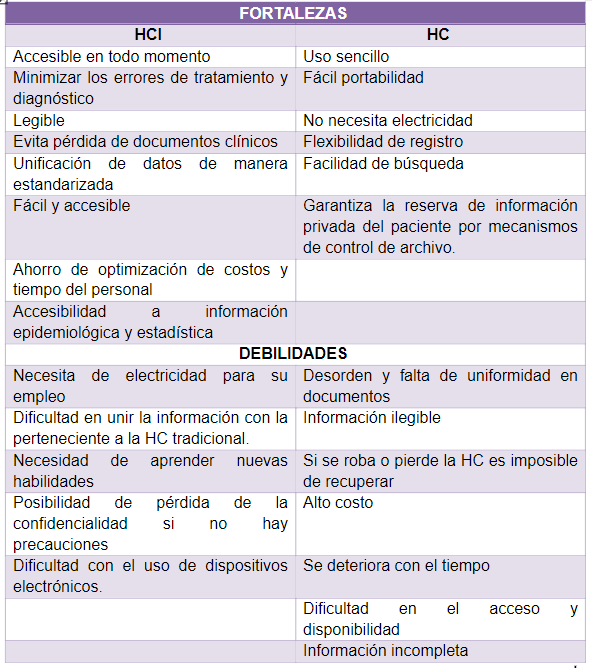
\includegraphics[]{MainMatter/HCIvsHC.PNG}
	\end{figure}
\end{center}

Ahora bien, todos los aspectos anteriormente descritos son superables mediante el desarrollo de las TIC, pero las fuentes primarias que nutren la construcción de la HCI es la actividad documentalista del equipo sanitario; sin su participación decidida para alimentar las bases de datos en forma adecuada no se lograrían los resultados esperados, constituyen el actor primario del proceso.  

\subsection{La HC en la medicina veterinaria}

Como mencionamos anteriormente la HCI no ha sido solo utilizada para atender a los seres humanos, sino que también se ha introducido en la medicina veterinaria. En la actualidad existen diferentes sitios online que se encargan de registrar y llevar la Historia Clínica Veterinaria (HCV) de sus animales. 

Entre los principales se encuentra la página web, la cual trabaja según el tipo de usuario que ingrese en el caso de dueño de una mascota o dedicado a la cría de animales, se registra como dueño de animal y se podrá ingresar todos los animales que quiera y llevar así la HC de cada uno. 

\textbf{QUE OTRAS APLICACIONES DE HCV EXISTEN EN EL PLANETA? PONER EJEMPLOS DE ALGUNAS MÓVILES}

\textbf{QUE EXISTE DE TODO ESTO EN CUBA}

\textbf{Esto abajo parece se refiere a la aplicación que se pretende desarrollar, o no? Si a mi no me quedó claro imaginen a los “de afuera”}

Este sistema se basa en que la propiedad de los datos es del dueño del animal, siendo muy útil para el veterinario que trate a tus animales actualmente, así como también para aquellos que los hagan en el futuro. 

El usuario dueño de animal, tiene dos opciones:  
\begin{enumerate}
\item ingresar la historia clínica el mismo, en caso que su veterinario no utilice este servicio,
\item esperar por la entrada de datos del veterinario y consultar los registros realizados por este.
\end{enumerate}
El otro usuario, el médico veterinario, tendrá a disposición de forma permanente la HC de sus pacientes y podrá ingresar datos como: motivos de consultas, alergias, vacunas y plan sanitario. Puede poseer al propio tiempo una agenda para la coordinación de consultas.  

Es importante decir que el sistema se basa en que las propiedades de los datos son del dueño del animal, y por este motivo, para que quede asentado en la HCV, una vez realizado el registro clínico por el veterinario, debe ser confirmado por el dueño del animal, esto lo hará en su próximo ingreso como usuario, ya que aparecerá una notificación donde se le preguntará si acepta el registro clínico del veterinario deseado, por cualquier motivo de consulta. Una vez confirmado estará disponible el registro clínico veterinario tanto para el dueño del animal como para él o los veterinarios que trabajen con la mascota. \brackcite{thesisSistemaInf}  
\newline
\newline

\textbf{{\large Conclusiones del Capítulo }}

\begin{enumerate}
	\item El bienestar animal es hoy una preocupación de la sociedad a nivel mundial; es por ello que se han adoptado estrategias interdisciplinarias y establecido leyes para protegerlos, así como se han aplicado los avances logrados en las TIC para mejorar la atención a estos seres vivos.  
	
	\item  Los servicios veterinarios datan de tiempos ancestrales, su evolución a través de la historia ha ido aparejada al propio desarrollo del ser humano. En Cuba ha experimentado un significativo progreso, siendo aprobado en el año anterior el Decreto-Ley No. 31 de Bienestar Animal. 
	
	\item La historia clínica veterinaria constituye un documento único confidencial e individual, en el cual queda plasmado el pronóstico, tratamiento y la evolución del paciente, de ahí la importancia de su correcta confección. 
	
	\item Las ciencias informáticas y bibliográficas han constituido un aporte significativo para el diseño y operación de los sistemas de información del sector sanitario, en especial de la HCI, la cual ha sido aplicada a la veterinaria mediante el desarrollo de sitios web. 
	
	\item La motivación, y capacitación del personal sanitario, el uso de las herramientas informáticas y de comunicación, y la toma de decisiones basada en evidencias demostrables, se convierten en la piedra angular de los servicios de atención veterinaria. 
\end{enumerate}